\documentclass[1p]{elsarticle_modified}
%\bibliographystyle{elsarticle-num}

%\usepackage[colorlinks]{hyperref}
%\usepackage{abbrmath_seonhwa} %\Abb, \Ascr, \Acal ,\Abf, \Afrak
\usepackage{amsfonts}
\usepackage{amssymb}
\usepackage{amsmath}
\usepackage{amsthm}
\usepackage{scalefnt}
\usepackage{amsbsy}
\usepackage{kotex}
\usepackage{caption}
\usepackage{subfig}
\usepackage{color}
\usepackage{graphicx}
\usepackage{xcolor} %% white, black, red, green, blue, cyan, magenta, yellow
\usepackage{float}
\usepackage{setspace}
\usepackage{hyperref}

\usepackage{tikz}
\usetikzlibrary{arrows}

\usepackage{multirow}
\usepackage{array} % fixed length table
\usepackage{hhline}

%%%%%%%%%%%%%%%%%%%%%
\makeatletter
\renewcommand*\env@matrix[1][\arraystretch]{%
	\edef\arraystretch{#1}%
	\hskip -\arraycolsep
	\let\@ifnextchar\new@ifnextchar
	\array{*\c@MaxMatrixCols c}}
\makeatother %https://tex.stackexchange.com/questions/14071/how-can-i-increase-the-line-spacing-in-a-matrix
%%%%%%%%%%%%%%%

\usepackage[normalem]{ulem}

\newcommand{\msout}[1]{\ifmmode\text{\sout{\ensuremath{#1}}}\else\sout{#1}\fi}
%SOURCE: \msout is \stkout macro in https://tex.stackexchange.com/questions/20609/strikeout-in-math-mode

\newcommand{\cancel}[1]{
	\ifmmode
	{\color{red}\msout{#1}}
	\else
	{\color{red}\sout{#1}}
	\fi
}

\newcommand{\add}[1]{
	{\color{blue}\uwave{#1}}
}

\newcommand{\replace}[2]{
	\ifmmode
	{\color{red}\msout{#1}}{\color{blue}\uwave{#2}}
	\else
	{\color{red}\sout{#1}}{\color{blue}\uwave{#2}}
	\fi
}

\newcommand{\Sol}{\mathcal{S}} %segment
\newcommand{\D}{D} %diagram
\newcommand{\A}{\mathcal{A}} %arc


%%%%%%%%%%%%%%%%%%%%%%%%%%%%%5 test

\def\sl{\operatorname{\textup{SL}}(2,\Cbb)}
\def\psl{\operatorname{\textup{PSL}}(2,\Cbb)}
\def\quan{\mkern 1mu \triangleright \mkern 1mu}

\theoremstyle{definition}
\newtheorem{thm}{Theorem}[section]
\newtheorem{prop}[thm]{Proposition}
\newtheorem{lem}[thm]{Lemma}
\newtheorem{ques}[thm]{Question}
\newtheorem{cor}[thm]{Corollary}
\newtheorem{defn}[thm]{Definition}
\newtheorem{exam}[thm]{Example}
\newtheorem{rmk}[thm]{Remark}
\newtheorem{alg}[thm]{Algorithm}

\newcommand{\I}{\sqrt{-1}}
\begin{document}

%\begin{frontmatter}
%
%\title{Boundary parabolic representations of knots up to 8 crossings}
%
%%% Group authors per affiliation:
%\author{Yunhi Cho} 
%\address{Department of Mathematics, University of Seoul, Seoul, Korea}
%\ead{yhcho@uos.ac.kr}
%
%
%\author{Seonhwa Kim} %\fnref{s_kim}}
%\address{Center for Geometry and Physics, Institute for Basic Science, Pohang, 37673, Korea}
%\ead{ryeona17@ibs.re.kr}
%
%\author{Hyuk Kim}
%\address{Department of Mathematical Sciences, Seoul National University, Seoul 08826, Korea}
%\ead{hyukkim@snu.ac.kr}
%
%\author{Seokbeom Yoon}
%\address{Department of Mathematical Sciences, Seoul National University, Seoul, 08826,  Korea}
%\ead{sbyoon15@snu.ac.kr}
%
%\begin{abstract}
%We find all boundary parabolic representation of knots up to 8 crossings.
%
%\end{abstract}
%\begin{keyword}
%    \MSC[2010] 57M25 
%\end{keyword}
%
%\end{frontmatter}

%\linenumbers
%\tableofcontents
%
\newcommand\colored[1]{\textcolor{white}{\rule[-0.35ex]{0.8em}{1.4ex}}\kern-0.8em\color{red} #1}%
%\newcommand\colored[1]{\textcolor{white}{ #1}\kern-2.17ex	\textcolor{white}{ #1}\kern-1.81ex	\textcolor{white}{ #1}\kern-2.15ex\color{red}#1	}

{\Large $\underline{11a_{233}~(K11a_{233})}$}

\setlength{\tabcolsep}{10pt}
\renewcommand{\arraystretch}{1.6}
\vspace{1cm}\begin{tabular}{m{100pt}>{\centering\arraybackslash}m{274pt}}
\multirow{5}{120pt}{
	\centering
	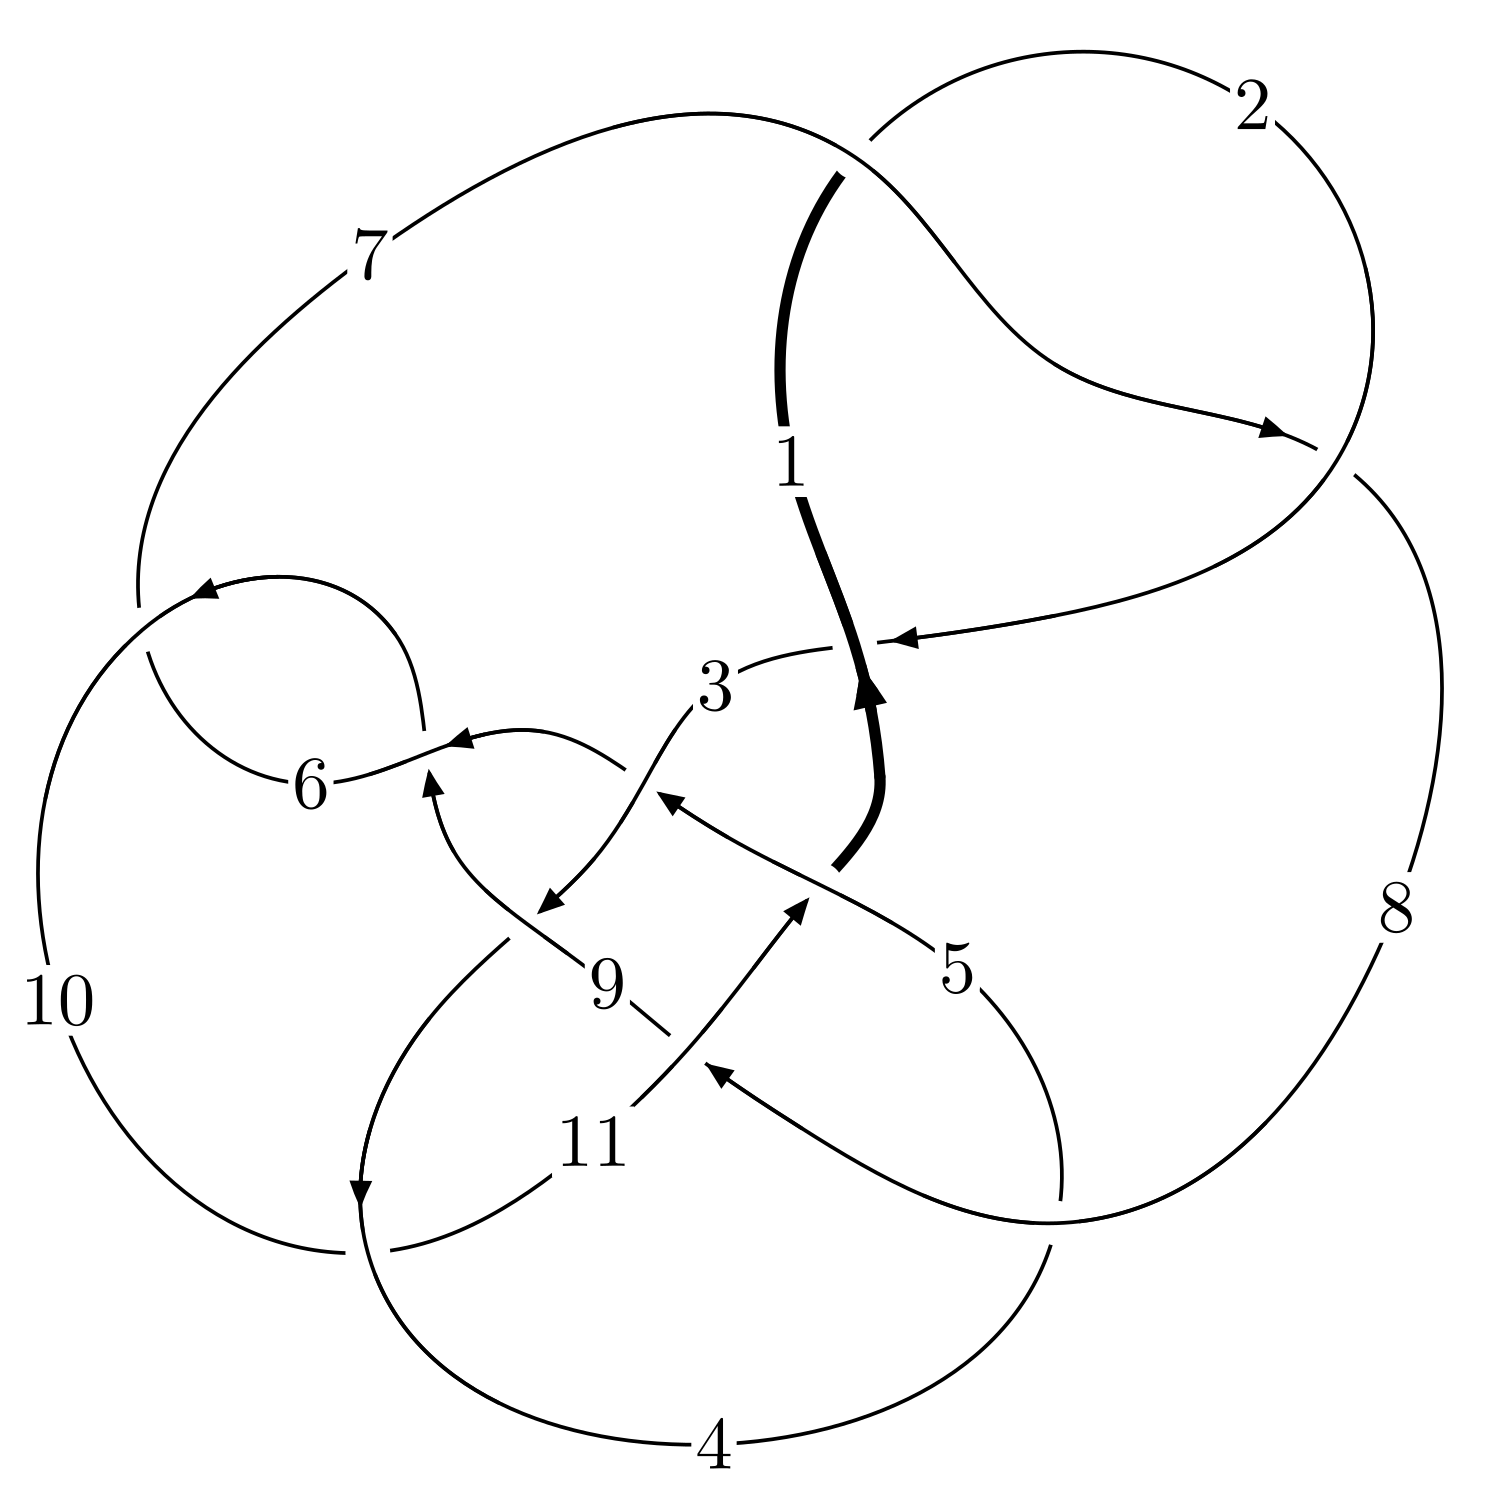
\includegraphics[width=112pt]{../../../GIT/diagram.site/Diagrams/png/482_11a_233.png}\\
\ \ \ A knot diagram\footnotemark}&
\allowdisplaybreaks
\textbf{Linearized knot diagam} \\
\cline{2-2}
 &
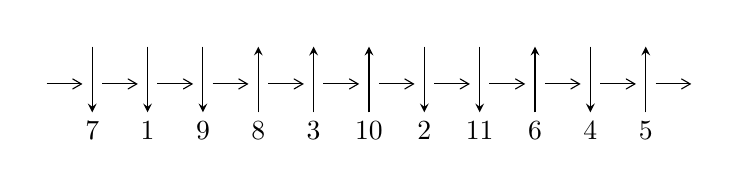
\begin{tikzpicture}[x=20pt, y=17pt]
	% nodes
	\node (C0) at (0, 0) {};
	\node (C1) at (1, 0) {};
	\node (C1U) at (1, +1) {};
	\node (C1D) at (1, -1) {7};

	\node (C2) at (2, 0) {};
	\node (C2U) at (2, +1) {};
	\node (C2D) at (2, -1) {1};

	\node (C3) at (3, 0) {};
	\node (C3U) at (3, +1) {};
	\node (C3D) at (3, -1) {9};

	\node (C4) at (4, 0) {};
	\node (C4U) at (4, +1) {};
	\node (C4D) at (4, -1) {8};

	\node (C5) at (5, 0) {};
	\node (C5U) at (5, +1) {};
	\node (C5D) at (5, -1) {3};

	\node (C6) at (6, 0) {};
	\node (C6U) at (6, +1) {};
	\node (C6D) at (6, -1) {10};

	\node (C7) at (7, 0) {};
	\node (C7U) at (7, +1) {};
	\node (C7D) at (7, -1) {2};

	\node (C8) at (8, 0) {};
	\node (C8U) at (8, +1) {};
	\node (C8D) at (8, -1) {11};

	\node (C9) at (9, 0) {};
	\node (C9U) at (9, +1) {};
	\node (C9D) at (9, -1) {6};

	\node (C10) at (10, 0) {};
	\node (C10U) at (10, +1) {};
	\node (C10D) at (10, -1) {4};

	\node (C11) at (11, 0) {};
	\node (C11U) at (11, +1) {};
	\node (C11D) at (11, -1) {5};
	\node (C12) at (12, 0) {};

	% arrows
	\draw[->,>={angle 60}]
	(C0) edge (C1) (C1) edge (C2) (C2) edge (C3) (C3) edge (C4) (C4) edge (C5) (C5) edge (C6) (C6) edge (C7) (C7) edge (C8) (C8) edge (C9) (C9) edge (C10) (C10) edge (C11) (C11) edge (C12) ;	\draw[->,>=stealth]
	(C1U) edge (C1D) (C2U) edge (C2D) (C3U) edge (C3D) (C4D) edge (C4U) (C5D) edge (C5U) (C6D) edge (C6U) (C7U) edge (C7D) (C8U) edge (C8D) (C9D) edge (C9U) (C10U) edge (C10D) (C11D) edge (C11U) ;
	\end{tikzpicture} \\
\hhline{~~} \\& 
\textbf{Solving Sequence} \\ \cline{2-2} 
 &
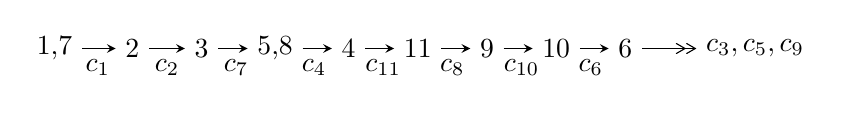
\begin{tikzpicture}[x=25pt, y=7pt]
	% node
	\node (A0) at (-1/8, 0) {1,7};
	\node (A1) at (1, 0) {2};
	\node (A2) at (2, 0) {3};
	\node (A3) at (49/16, 0) {5,8};
	\node (A4) at (33/8, 0) {4};
	\node (A5) at (41/8, 0) {11};
	\node (A6) at (49/8, 0) {9};
	\node (A7) at (57/8, 0) {10};
	\node (A8) at (65/8, 0) {6};
	\node (C1) at (1/2, -1) {$c_{1}$};
	\node (C2) at (3/2, -1) {$c_{2}$};
	\node (C3) at (5/2, -1) {$c_{7}$};
	\node (C4) at (29/8, -1) {$c_{4}$};
	\node (C5) at (37/8, -1) {$c_{11}$};
	\node (C6) at (45/8, -1) {$c_{8}$};
	\node (C7) at (53/8, -1) {$c_{10}$};
	\node (C8) at (61/8, -1) {$c_{6}$};
	\node (A9) at (10, 0) {$c_{3},c_{5},c_{9}$};

	% edge
	\draw[->,>=stealth]	
	(A0) edge (A1) (A1) edge (A2) (A2) edge (A3) (A3) edge (A4) (A4) edge (A5) (A5) edge (A6) (A6) edge (A7) (A7) edge (A8) ;
	\draw[->>,>={angle 60}]	
	(A8) edge (A9);
\end{tikzpicture} \\ 

\end{tabular} \\

\footnotetext{
The image of knot diagram is generated by the software ``\textbf{Draw programme}" developed by Andrew Bartholomew(\url{http://www.layer8.co.uk/maths/draw/index.htm\#Running-draw}), where we modified some parts for our purpose(\url{https://github.com/CATsTAILs/LinksPainter}).
}\phantom \\ \newline 
\centering \textbf{Ideals for irreducible components\footnotemark of $X_{\text{par}}$} 
 
\begin{align*}
I^u_{1}&=\langle 
-2.27632\times10^{208} u^{109}+1.94112\times10^{208} u^{108}+\cdots+4.24838\times10^{207} b+1.02341\times10^{210},\\
\phantom{I^u_{1}}&\phantom{= \langle  }-3.37601\times10^{209} u^{109}+7.54876\times10^{209} u^{108}+\cdots+2.08171\times10^{209} a-4.18256\times10^{210},\\
\phantom{I^u_{1}}&\phantom{= \langle  }u^{110}-25 u^{108}+\cdots-111 u-49\rangle \\
I^u_{2}&=\langle 
- u^{23}- u^{22}+\cdots+b+1,\;213 u^{23}+206 u^{22}+\cdots+19 a-309,\;u^{24}+u^{23}+\cdots-4 u-1\rangle \\
\\
\end{align*}
\raggedright * 2 irreducible components of $\dim_{\mathbb{C}}=0$, with total 134 representations.\\
\footnotetext{All coefficients of polynomials are rational numbers. But the coefficients are sometimes approximated in decimal forms when there is not enough margin.}
\newpage
\renewcommand{\arraystretch}{1}
\centering \section*{I. $I^u_{1}= \langle -2.28\times10^{208} u^{109}+1.94\times10^{208} u^{108}+\cdots+4.25\times10^{207} b+1.02\times10^{210},\;-3.38\times10^{209} u^{109}+7.55\times10^{209} u^{108}+\cdots+2.08\times10^{209} a-4.18\times10^{210},\;u^{110}-25 u^{108}+\cdots-111 u-49 \rangle$}
\flushleft \textbf{(i) Arc colorings}\\
\begin{tabular}{m{7pt} m{180pt} m{7pt} m{180pt} }
\flushright $a_{1}=$&$\begin{pmatrix}1\\0\end{pmatrix}$ \\
\flushright $a_{7}=$&$\begin{pmatrix}0\\u\end{pmatrix}$ \\
\flushright $a_{2}=$&$\begin{pmatrix}1\\u^2\end{pmatrix}$ \\
\flushright $a_{3}=$&$\begin{pmatrix}- u^2+1\\u^2\end{pmatrix}$ \\
\flushright $a_{5}=$&$\begin{pmatrix}1.62175 u^{109}-3.62623 u^{108}+\cdots-57.1057 u+20.0920\\5.35809 u^{109}-4.56908 u^{108}+\cdots-399.860 u-240.893\end{pmatrix}$ \\
\flushright $a_{8}=$&$\begin{pmatrix}- u\\- u^3+u\end{pmatrix}$ \\
\flushright $a_{4}=$&$\begin{pmatrix}-1.91012 u^{109}-0.808931 u^{108}+\cdots+191.146 u+188.961\\7.74510 u^{109}-7.62401 u^{108}+\cdots-508.453 u-271.714\end{pmatrix}$ \\
\flushright $a_{11}=$&$\begin{pmatrix}-6.62292 u^{109}+6.81033 u^{108}+\cdots+447.228 u+250.503\\3.00556 u^{109}-6.70861 u^{108}+\cdots-105.567 u+75.2016\end{pmatrix}$ \\
\flushright $a_{9}=$&$\begin{pmatrix}8.05410 u^{109}-8.44201 u^{108}+\cdots-548.617 u-273.571\\-1.92264 u^{109}+8.03692 u^{108}+\cdots-20.2333 u-246.169\end{pmatrix}$ \\
\flushright $a_{10}=$&$\begin{pmatrix}-5.59038 u^{109}+4.91305 u^{108}+\cdots+389.785 u+244.009\\4.07996 u^{109}-8.62390 u^{108}+\cdots-159.703 u+79.3119\end{pmatrix}$ \\
\flushright $a_{6}=$&$\begin{pmatrix}-1.66281 u^{109}-0.839116 u^{108}+\cdots+171.874 u+172.557\\7.01460 u^{109}-7.18860 u^{108}+\cdots-461.032 u-232.681\end{pmatrix}$\\ \flushright $a_{6}=$&$\begin{pmatrix}-1.66281 u^{109}-0.839116 u^{108}+\cdots+171.874 u+172.557\\7.01460 u^{109}-7.18860 u^{108}+\cdots-461.032 u-232.681\end{pmatrix}$\\&\end{tabular}
\flushleft \textbf{(ii) Obstruction class $= -1$}\\~\\
\flushleft \textbf{(iii) Cusp Shapes $= -8.45708 u^{109}+8.40205 u^{108}+\cdots+589.854 u+392.471$}\\~\\
\newpage\renewcommand{\arraystretch}{1}
\flushleft \textbf{(iv) u-Polynomials at the component}\newline \\
\begin{tabular}{m{50pt}|m{274pt}}
Crossings & \hspace{64pt}u-Polynomials at each crossing \\
\hline $$\begin{aligned}c_{1},c_{7}\end{aligned}$$&$\begin{aligned}
&u^{110}-25 u^{108}+\cdots+111 u-49
\end{aligned}$\\
\hline $$\begin{aligned}c_{2}\end{aligned}$$&$\begin{aligned}
&u^{110}+50 u^{109}+\cdots+26237 u+2401
\end{aligned}$\\
\hline $$\begin{aligned}c_{3}\end{aligned}$$&$\begin{aligned}
&u^{110}- u^{109}+\cdots-33999 u-6849
\end{aligned}$\\
\hline $$\begin{aligned}c_{4}\end{aligned}$$&$\begin{aligned}
&u^{110}-3 u^{109}+\cdots-41 u-1
\end{aligned}$\\
\hline $$\begin{aligned}c_{5}\end{aligned}$$&$\begin{aligned}
&u^{110}-7 u^{109}+\cdots-126089 u-152261
\end{aligned}$\\
\hline $$\begin{aligned}c_{6},c_{9}\end{aligned}$$&$\begin{aligned}
&u^{110}-33 u^{108}+\cdots-32 u+1133
\end{aligned}$\\
\hline $$\begin{aligned}c_{8}\end{aligned}$$&$\begin{aligned}
&u^{110}-9 u^{109}+\cdots+21 u-1
\end{aligned}$\\
\hline $$\begin{aligned}c_{10}\end{aligned}$$&$\begin{aligned}
&u^{110}+3 u^{109}+\cdots-37 u+1
\end{aligned}$\\
\hline $$\begin{aligned}c_{11}\end{aligned}$$&$\begin{aligned}
&u^{110}-5 u^{108}+\cdots+5654 u-1721
\end{aligned}$\\
\hline
\end{tabular}\\~\\
\newpage\renewcommand{\arraystretch}{1}
\flushleft \textbf{(v) Riley Polynomials at the component}\newline \\
\begin{tabular}{m{50pt}|m{274pt}}
Crossings & \hspace{64pt}Riley Polynomials at each crossing \\
\hline $$\begin{aligned}c_{1},c_{7}\end{aligned}$$&$\begin{aligned}
&y^{110}-50 y^{109}+\cdots-26237 y+2401
\end{aligned}$\\
\hline $$\begin{aligned}c_{2}\end{aligned}$$&$\begin{aligned}
&y^{110}+30 y^{109}+\cdots-18049781 y+5764801
\end{aligned}$\\
\hline $$\begin{aligned}c_{3}\end{aligned}$$&$\begin{aligned}
&y^{110}+21 y^{109}+\cdots+2263623021 y+46908801
\end{aligned}$\\
\hline $$\begin{aligned}c_{4}\end{aligned}$$&$\begin{aligned}
&y^{110}+y^{109}+\cdots-205 y+1
\end{aligned}$\\
\hline $$\begin{aligned}c_{5}\end{aligned}$$&$\begin{aligned}
&y^{110}-35 y^{109}+\cdots+362704631019 y+23183412121
\end{aligned}$\\
\hline $$\begin{aligned}c_{6},c_{9}\end{aligned}$$&$\begin{aligned}
&y^{110}-66 y^{109}+\cdots-31330740 y+1283689
\end{aligned}$\\
\hline $$\begin{aligned}c_{8}\end{aligned}$$&$\begin{aligned}
&y^{110}+y^{109}+\cdots+19 y+1
\end{aligned}$\\
\hline $$\begin{aligned}c_{10}\end{aligned}$$&$\begin{aligned}
&y^{110}+5 y^{109}+\cdots-129 y+1
\end{aligned}$\\
\hline $$\begin{aligned}c_{11}\end{aligned}$$&$\begin{aligned}
&y^{110}-10 y^{109}+\cdots-173719602 y+2961841
\end{aligned}$\\
\hline
\end{tabular}\\~\\
\newpage\flushleft \textbf{(vi) Complex Volumes and Cusp Shapes}
$$\begin{array}{c|c|c}  
\text{Solutions to }I^u_{1}& \I (\text{vol} + \sqrt{-1}CS) & \text{Cusp shape}\\
 \hline 
\begin{aligned}
u &= -0.877207 + 0.464777 I \\
a &= -1.63345 - 0.65594 I \\
b &= -0.30513 + 2.32582 I\end{aligned}
 & -2.81741 + 1.89701 I & \phantom{-0.000000 } 0 \\ \hline\begin{aligned}
u &= -0.877207 - 0.464777 I \\
a &= -1.63345 + 0.65594 I \\
b &= -0.30513 - 2.32582 I\end{aligned}
 & -2.81741 - 1.89701 I & \phantom{-0.000000 } 0 \\ \hline\begin{aligned}
u &= -0.906253 + 0.459377 I \\
a &= -0.216830 - 0.375187 I \\
b &= \phantom{-}0.074681 - 1.025680 I\end{aligned}
 & -1.38141 + 4.57448 I & \phantom{-0.000000 } 0 \\ \hline\begin{aligned}
u &= -0.906253 - 0.459377 I \\
a &= -0.216830 + 0.375187 I \\
b &= \phantom{-}0.074681 + 1.025680 I\end{aligned}
 & -1.38141 - 4.57448 I & \phantom{-0.000000 } 0 \\ \hline\begin{aligned}
u &= \phantom{-}0.779379 + 0.592089 I \\
a &= -1.16698 - 1.53479 I \\
b &= \phantom{-}0.815736 - 0.623391 I\end{aligned}
 & \phantom{-}4.64623 - 0.04743 I & \phantom{-0.000000 } 0 \\ \hline\begin{aligned}
u &= \phantom{-}0.779379 - 0.592089 I \\
a &= -1.16698 + 1.53479 I \\
b &= \phantom{-}0.815736 + 0.623391 I\end{aligned}
 & \phantom{-}4.64623 + 0.04743 I & \phantom{-0.000000 } 0 \\ \hline\begin{aligned}
u &= -0.862031 + 0.455176 I \\
a &= \phantom{-}0.603643 - 0.885853 I \\
b &= \phantom{-}0.378364 - 1.127920 I\end{aligned}
 & -1.23201 - 0.85043 I & \phantom{-0.000000 } 0 \\ \hline\begin{aligned}
u &= -0.862031 - 0.455176 I \\
a &= \phantom{-}0.603643 + 0.885853 I \\
b &= \phantom{-}0.378364 + 1.127920 I\end{aligned}
 & -1.23201 + 0.85043 I & \phantom{-0.000000 } 0 \\ \hline\begin{aligned}
u &= \phantom{-}0.498633 + 0.834333 I \\
a &= -1.24445 - 1.05722 I \\
b &= \phantom{-}1.30739 + 0.77834 I\end{aligned}
 & \phantom{-}2.08576 + 6.71841 I & \phantom{-0.000000 } 0 \\ \hline\begin{aligned}
u &= \phantom{-}0.498633 - 0.834333 I \\
a &= -1.24445 + 1.05722 I \\
b &= \phantom{-}1.30739 - 0.77834 I\end{aligned}
 & \phantom{-}2.08576 - 6.71841 I & \phantom{-0.000000 } 0\\
 \hline 
 \end{array}$$\newpage$$\begin{array}{c|c|c}  
\text{Solutions to }I^u_{1}& \I (\text{vol} + \sqrt{-1}CS) & \text{Cusp shape}\\
 \hline 
\begin{aligned}
u &= -0.919272 + 0.312694 I \\
a &= \phantom{-}2.30721 - 0.99992 I \\
b &= -1.27590 - 1.00769 I\end{aligned}
 & \phantom{-}0.29208 - 3.63942 I & \phantom{-0.000000 } 0 \\ \hline\begin{aligned}
u &= -0.919272 - 0.312694 I \\
a &= \phantom{-}2.30721 + 0.99992 I \\
b &= -1.27590 + 1.00769 I\end{aligned}
 & \phantom{-}0.29208 + 3.63942 I & \phantom{-0.000000 } 0 \\ \hline\begin{aligned}
u &= \phantom{-}0.894461 + 0.341485 I \\
a &= -0.458154 - 0.689277 I \\
b &= \phantom{-}0.790844 + 0.231478 I\end{aligned}
 & -1.66024 - 0.89300 I & \phantom{-0.000000 } 0 \\ \hline\begin{aligned}
u &= \phantom{-}0.894461 - 0.341485 I \\
a &= -0.458154 + 0.689277 I \\
b &= \phantom{-}0.790844 - 0.231478 I\end{aligned}
 & -1.66024 + 0.89300 I & \phantom{-0.000000 } 0 \\ \hline\begin{aligned}
u &= \phantom{-}0.699495 + 0.780649 I \\
a &= \phantom{-}1.198460 - 0.366427 I \\
b &= -0.793614 - 0.327881 I\end{aligned}
 & \phantom{-}6.12266 + 3.41032 I & \phantom{-0.000000 } 0 \\ \hline\begin{aligned}
u &= \phantom{-}0.699495 - 0.780649 I \\
a &= \phantom{-}1.198460 + 0.366427 I \\
b &= -0.793614 + 0.327881 I\end{aligned}
 & \phantom{-}6.12266 - 3.41032 I & \phantom{-0.000000 } 0 \\ \hline\begin{aligned}
u &= \phantom{-}0.908401 + 0.528181 I \\
a &= -2.28390 - 0.15768 I \\
b &= \phantom{-}0.732017 - 0.538186 I\end{aligned}
 & -0.65779 - 5.16179 I & \phantom{-0.000000 } 0 \\ \hline\begin{aligned}
u &= \phantom{-}0.908401 - 0.528181 I \\
a &= -2.28390 + 0.15768 I \\
b &= \phantom{-}0.732017 + 0.538186 I\end{aligned}
 & -0.65779 + 5.16179 I & \phantom{-0.000000 } 0 \\ \hline\begin{aligned}
u &= -0.450080 + 0.954070 I \\
a &= -1.21322 + 0.77988 I \\
b &= \phantom{-}1.31650 - 0.83984 I\end{aligned}
 & \phantom{-}6.1363 - 12.7818 I & \phantom{-0.000000 } 0 \\ \hline\begin{aligned}
u &= -0.450080 - 0.954070 I \\
a &= -1.21322 - 0.77988 I \\
b &= \phantom{-}1.31650 + 0.83984 I\end{aligned}
 & \phantom{-}6.1363 + 12.7818 I & \phantom{-0.000000 } 0\\
 \hline 
 \end{array}$$\newpage$$\begin{array}{c|c|c}  
\text{Solutions to }I^u_{1}& \I (\text{vol} + \sqrt{-1}CS) & \text{Cusp shape}\\
 \hline 
\begin{aligned}
u &= \phantom{-}0.933669 + 0.499305 I \\
a &= \phantom{-}1.95385 + 0.36470 I \\
b &= -1.00796 + 1.26733 I\end{aligned}
 & -2.36919 - 2.67543 I & \phantom{-0.000000 } 0 \\ \hline\begin{aligned}
u &= \phantom{-}0.933669 - 0.499305 I \\
a &= \phantom{-}1.95385 - 0.36470 I \\
b &= -1.00796 - 1.26733 I\end{aligned}
 & -2.36919 + 2.67543 I & \phantom{-0.000000 } 0 \\ \hline\begin{aligned}
u &= -0.928488 + 0.102480 I \\
a &= \phantom{-}1.60356 - 0.71634 I \\
b &= \phantom{-}0.492832 - 0.757582 I\end{aligned}
 & \phantom{-}1.78332 - 2.50693 I & \phantom{-0.000000 } 0 \\ \hline\begin{aligned}
u &= -0.928488 - 0.102480 I \\
a &= \phantom{-}1.60356 + 0.71634 I \\
b &= \phantom{-}0.492832 + 0.757582 I\end{aligned}
 & \phantom{-}1.78332 + 2.50693 I & \phantom{-0.000000 } 0 \\ \hline\begin{aligned}
u &= \phantom{-}1.015960 + 0.327336 I \\
a &= \phantom{-}0.403514 - 0.415868 I \\
b &= \phantom{-}0.712743 + 0.871977 I\end{aligned}
 & -1.96403 - 0.96664 I & \phantom{-0.000000 } 0 \\ \hline\begin{aligned}
u &= \phantom{-}1.015960 - 0.327336 I \\
a &= \phantom{-}0.403514 + 0.415868 I \\
b &= \phantom{-}0.712743 - 0.871977 I\end{aligned}
 & -1.96403 + 0.96664 I & \phantom{-0.000000 } 0 \\ \hline\begin{aligned}
u &= \phantom{-}0.906000 + 0.578199 I \\
a &= \phantom{-}1.032450 + 0.199832 I \\
b &= -1.186720 - 0.508749 I\end{aligned}
 & \phantom{-}4.25014 - 4.59723 I & \phantom{-0.000000 } 0 \\ \hline\begin{aligned}
u &= \phantom{-}0.906000 - 0.578199 I \\
a &= \phantom{-}1.032450 - 0.199832 I \\
b &= -1.186720 + 0.508749 I\end{aligned}
 & \phantom{-}4.25014 + 4.59723 I & \phantom{-0.000000 } 0 \\ \hline\begin{aligned}
u &= -1.069320 + 0.108926 I \\
a &= -0.483978 + 0.417342 I \\
b &= \phantom{-}0.183669 + 1.073570 I\end{aligned}
 & -5.09720 + 2.43411 I & \phantom{-0.000000 } 0 \\ \hline\begin{aligned}
u &= -1.069320 - 0.108926 I \\
a &= -0.483978 - 0.417342 I \\
b &= \phantom{-}0.183669 - 1.073570 I\end{aligned}
 & -5.09720 - 2.43411 I & \phantom{-0.000000 } 0\\
 \hline 
 \end{array}$$\newpage$$\begin{array}{c|c|c}  
\text{Solutions to }I^u_{1}& \I (\text{vol} + \sqrt{-1}CS) & \text{Cusp shape}\\
 \hline 
\begin{aligned}
u &= \phantom{-}0.768096 + 0.504247 I \\
a &= \phantom{-}1.10361 + 1.56209 I \\
b &= -0.403494 - 0.242985 I\end{aligned}
 & -0.213297 + 0.928435 I & \phantom{-0.000000 } 0 \\ \hline\begin{aligned}
u &= \phantom{-}0.768096 - 0.504247 I \\
a &= \phantom{-}1.10361 - 1.56209 I \\
b &= -0.403494 + 0.242985 I\end{aligned}
 & -0.213297 - 0.928435 I & \phantom{-0.000000 } 0 \\ \hline\begin{aligned}
u &= -0.693726 + 0.829558 I \\
a &= -0.779769 + 1.106130 I \\
b &= \phantom{-}1.31216 - 0.72509 I\end{aligned}
 & \phantom{-}7.43132 - 0.79593 I & \phantom{-0.000000 } 0 \\ \hline\begin{aligned}
u &= -0.693726 - 0.829558 I \\
a &= -0.779769 - 1.106130 I \\
b &= \phantom{-}1.31216 + 0.72509 I\end{aligned}
 & \phantom{-}7.43132 + 0.79593 I & \phantom{-0.000000 } 0 \\ \hline\begin{aligned}
u &= \phantom{-}0.523668 + 0.741211 I \\
a &= \phantom{-}1.12373 + 0.96400 I \\
b &= -1.42277 - 1.05594 I\end{aligned}
 & \phantom{-}6.62680 + 3.46904 I & \phantom{-0.000000 } 0 \\ \hline\begin{aligned}
u &= \phantom{-}0.523668 - 0.741211 I \\
a &= \phantom{-}1.12373 - 0.96400 I \\
b &= -1.42277 + 1.05594 I\end{aligned}
 & \phantom{-}6.62680 - 3.46904 I & \phantom{-0.000000 } 0 \\ \hline\begin{aligned}
u &= \phantom{-}0.378004 + 0.807900 I \\
a &= -0.378489 + 0.463144 I \\
b &= \phantom{-}0.682090 - 0.070661 I\end{aligned}
 & \phantom{-}1.72185 - 3.26106 I & \phantom{-0.000000 } 0 \\ \hline\begin{aligned}
u &= \phantom{-}0.378004 - 0.807900 I \\
a &= -0.378489 - 0.463144 I \\
b &= \phantom{-}0.682090 + 0.070661 I\end{aligned}
 & \phantom{-}1.72185 + 3.26106 I & \phantom{-0.000000 } 0 \\ \hline\begin{aligned}
u &= -0.795267 + 0.389203 I \\
a &= \phantom{-}1.76374 - 0.04444 I \\
b &= -1.208800 + 0.171994 I\end{aligned}
 & \phantom{-}2.92619 - 0.62432 I & \phantom{-0.000000 } 0 \\ \hline\begin{aligned}
u &= -0.795267 - 0.389203 I \\
a &= \phantom{-}1.76374 + 0.04444 I \\
b &= -1.208800 - 0.171994 I\end{aligned}
 & \phantom{-}2.92619 + 0.62432 I & \phantom{-0.000000 } 0\\
 \hline 
 \end{array}$$\newpage$$\begin{array}{c|c|c}  
\text{Solutions to }I^u_{1}& \I (\text{vol} + \sqrt{-1}CS) & \text{Cusp shape}\\
 \hline 
\begin{aligned}
u &= -0.963056 + 0.572158 I \\
a &= -0.92650 + 1.41091 I \\
b &= \phantom{-}0.749621 + 0.384131 I\end{aligned}
 & \phantom{-}1.67436 + 4.68049 I & \phantom{-0.000000 } 0 \\ \hline\begin{aligned}
u &= -0.963056 - 0.572158 I \\
a &= -0.92650 - 1.41091 I \\
b &= \phantom{-}0.749621 - 0.384131 I\end{aligned}
 & \phantom{-}1.67436 - 4.68049 I & \phantom{-0.000000 } 0 \\ \hline\begin{aligned}
u &= -0.449330 + 1.028380 I \\
a &= -0.468032 + 0.389341 I \\
b &= \phantom{-}0.773402 - 0.518641 I\end{aligned}
 & \phantom{-}4.82382 - 4.21742 I & \phantom{-0.000000 } 0 \\ \hline\begin{aligned}
u &= -0.449330 - 1.028380 I \\
a &= -0.468032 - 0.389341 I \\
b &= \phantom{-}0.773402 + 0.518641 I\end{aligned}
 & \phantom{-}4.82382 + 4.21742 I & \phantom{-0.000000 } 0 \\ \hline\begin{aligned}
u &= \phantom{-}0.977137 + 0.554900 I \\
a &= -0.975120 + 0.865655 I \\
b &= -0.82789 - 2.04963 I\end{aligned}
 & \phantom{-}1.86655 - 8.96327 I & \phantom{-0.000000 } 0 \\ \hline\begin{aligned}
u &= \phantom{-}0.977137 - 0.554900 I \\
a &= -0.975120 - 0.865655 I \\
b &= -0.82789 + 2.04963 I\end{aligned}
 & \phantom{-}1.86655 + 8.96327 I & \phantom{-0.000000 } 0 \\ \hline\begin{aligned}
u &= \phantom{-}0.347166 + 0.792807 I \\
a &= \phantom{-}1.176620 - 0.063753 I \\
b &= -1.353060 + 0.254781 I\end{aligned}
 & \phantom{-}5.78414 - 0.80826 I & \phantom{-0.000000 } 0 \\ \hline\begin{aligned}
u &= \phantom{-}0.347166 - 0.792807 I \\
a &= \phantom{-}1.176620 + 0.063753 I \\
b &= -1.353060 - 0.254781 I\end{aligned}
 & \phantom{-}5.78414 + 0.80826 I & \phantom{-0.000000 } 0 \\ \hline\begin{aligned}
u &= \phantom{-}1.077080 + 0.357090 I \\
a &= \phantom{-}0.496904 + 0.747927 I \\
b &= \phantom{-}0.562525 + 1.139530 I\end{aligned}
 & -1.19948 + 1.82986 I & \phantom{-0.000000 } 0 \\ \hline\begin{aligned}
u &= \phantom{-}1.077080 - 0.357090 I \\
a &= \phantom{-}0.496904 - 0.747927 I \\
b &= \phantom{-}0.562525 - 1.139530 I\end{aligned}
 & -1.19948 - 1.82986 I & \phantom{-0.000000 } 0\\
 \hline 
 \end{array}$$\newpage$$\begin{array}{c|c|c}  
\text{Solutions to }I^u_{1}& \I (\text{vol} + \sqrt{-1}CS) & \text{Cusp shape}\\
 \hline 
\begin{aligned}
u &= \phantom{-}0.554814 + 1.000080 I \\
a &= \phantom{-}1.093360 + 0.477457 I \\
b &= -0.980163 - 0.369618 I\end{aligned}
 & \phantom{-}2.97612 + 3.19519 I & \phantom{-0.000000 } 0 \\ \hline\begin{aligned}
u &= \phantom{-}0.554814 - 1.000080 I \\
a &= \phantom{-}1.093360 - 0.477457 I \\
b &= -0.980163 + 0.369618 I\end{aligned}
 & \phantom{-}2.97612 - 3.19519 I & \phantom{-0.000000 } 0 \\ \hline\begin{aligned}
u &= -1.149670 + 0.046838 I \\
a &= -0.399836 + 0.038087 I \\
b &= -0.692479 + 0.940995 I\end{aligned}
 & -3.72221 - 4.85234 I & \phantom{-0.000000 } 0 \\ \hline\begin{aligned}
u &= -1.149670 - 0.046838 I \\
a &= -0.399836 - 0.038087 I \\
b &= -0.692479 - 0.940995 I\end{aligned}
 & -3.72221 + 4.85234 I & \phantom{-0.000000 } 0 \\ \hline\begin{aligned}
u &= -0.310587 + 0.786939 I \\
a &= \phantom{-}1.51809 - 0.41405 I \\
b &= -0.953194 + 0.420891 I\end{aligned}
 & \phantom{-}1.63201 - 1.67537 I & \phantom{-0.000000 } 0 \\ \hline\begin{aligned}
u &= -0.310587 - 0.786939 I \\
a &= \phantom{-}1.51809 + 0.41405 I \\
b &= -0.953194 - 0.420891 I\end{aligned}
 & \phantom{-}1.63201 + 1.67537 I & \phantom{-0.000000 } 0 \\ \hline\begin{aligned}
u &= \phantom{-}0.657188 + 0.523339 I \\
a &= -1.76810 + 0.26229 I \\
b &= \phantom{-}0.25935 - 1.89224 I\end{aligned}
 & \phantom{-}2.86926 + 4.53794 I & \phantom{-0.000000 } 0 \\ \hline\begin{aligned}
u &= \phantom{-}0.657188 - 0.523339 I \\
a &= -1.76810 - 0.26229 I \\
b &= \phantom{-}0.25935 + 1.89224 I\end{aligned}
 & \phantom{-}2.86926 - 4.53794 I & \phantom{-0.000000 } 0 \\ \hline\begin{aligned}
u &= -0.576594 + 0.605519 I \\
a &= \phantom{-}1.356830 + 0.270002 I \\
b &= -0.953112 + 0.084959 I\end{aligned}
 & \phantom{-}2.76606 - 0.05036 I & \phantom{-0.000000 } 0 \\ \hline\begin{aligned}
u &= -0.576594 - 0.605519 I \\
a &= \phantom{-}1.356830 - 0.270002 I \\
b &= -0.953112 - 0.084959 I\end{aligned}
 & \phantom{-}2.76606 + 0.05036 I & \phantom{-0.000000 } 0\\
 \hline 
 \end{array}$$\newpage$$\begin{array}{c|c|c}  
\text{Solutions to }I^u_{1}& \I (\text{vol} + \sqrt{-1}CS) & \text{Cusp shape}\\
 \hline 
\begin{aligned}
u &= -1.052560 + 0.500476 I \\
a &= -2.18256 + 1.04458 I \\
b &= \phantom{-}0.709599 + 0.809395 I\end{aligned}
 & -0.29158 + 8.70811 I & \phantom{-0.000000 } 0 \\ \hline\begin{aligned}
u &= -1.052560 - 0.500476 I \\
a &= -2.18256 - 1.04458 I \\
b &= \phantom{-}0.709599 - 0.809395 I\end{aligned}
 & -0.29158 - 8.70811 I & \phantom{-0.000000 } 0 \\ \hline\begin{aligned}
u &= -1.062770 + 0.482900 I \\
a &= -0.855928 + 0.673982 I \\
b &= \phantom{-}0.585258 - 0.115320 I\end{aligned}
 & -0.74609 + 5.32896 I & \phantom{-0.000000 } 0 \\ \hline\begin{aligned}
u &= -1.062770 - 0.482900 I \\
a &= -0.855928 - 0.673982 I \\
b &= \phantom{-}0.585258 + 0.115320 I\end{aligned}
 & -0.74609 - 5.32896 I & \phantom{-0.000000 } 0 \\ \hline\begin{aligned}
u &= -1.072460 + 0.462666 I \\
a &= -1.12860 + 1.34169 I \\
b &= \phantom{-}1.45190 + 0.29838 I\end{aligned}
 & -0.96350 + 5.88120 I & \phantom{-0.000000 } 0 \\ \hline\begin{aligned}
u &= -1.072460 - 0.462666 I \\
a &= -1.12860 - 1.34169 I \\
b &= \phantom{-}1.45190 - 0.29838 I\end{aligned}
 & -0.96350 - 5.88120 I & \phantom{-0.000000 } 0 \\ \hline\begin{aligned}
u &= -1.096870 + 0.405245 I \\
a &= -0.295230 + 1.369570 I \\
b &= \phantom{-}1.046210 + 0.360865 I\end{aligned}
 & \phantom{-}1.77521 + 3.72119 I & \phantom{-0.000000 } 0 \\ \hline\begin{aligned}
u &= -1.096870 - 0.405245 I \\
a &= -0.295230 - 1.369570 I \\
b &= \phantom{-}1.046210 - 0.360865 I\end{aligned}
 & \phantom{-}1.77521 - 3.72119 I & \phantom{-0.000000 } 0 \\ \hline\begin{aligned}
u &= -0.665044 + 0.962961 I \\
a &= -0.869511 - 0.020998 I \\
b &= \phantom{-}1.001420 + 0.089018 I\end{aligned}
 & \phantom{-}7.39423 + 7.45324 I & \phantom{-0.000000 } 0 \\ \hline\begin{aligned}
u &= -0.665044 - 0.962961 I \\
a &= -0.869511 + 0.020998 I \\
b &= \phantom{-}1.001420 - 0.089018 I\end{aligned}
 & \phantom{-}7.39423 - 7.45324 I & \phantom{-0.000000 } 0\\
 \hline 
 \end{array}$$\newpage$$\begin{array}{c|c|c}  
\text{Solutions to }I^u_{1}& \I (\text{vol} + \sqrt{-1}CS) & \text{Cusp shape}\\
 \hline 
\begin{aligned}
u &= \phantom{-}0.986287 + 0.678798 I \\
a &= -1.04231 - 1.40120 I \\
b &= \phantom{-}0.591393 - 0.442123 I\end{aligned}
 & \phantom{-}5.22686 - 8.92615 I & \phantom{-0.000000 } 0 \\ \hline\begin{aligned}
u &= \phantom{-}0.986287 - 0.678798 I \\
a &= -1.04231 + 1.40120 I \\
b &= \phantom{-}0.591393 + 0.442123 I\end{aligned}
 & \phantom{-}5.22686 + 8.92615 I & \phantom{-0.000000 } 0 \\ \hline\begin{aligned}
u &= -0.985417 + 0.709019 I \\
a &= \phantom{-}1.66661 - 0.54822 I \\
b &= -1.37059 - 1.09406 I\end{aligned}
 & \phantom{-}6.52722 + 6.52907 I & \phantom{-0.000000 } 0 \\ \hline\begin{aligned}
u &= -0.985417 - 0.709019 I \\
a &= \phantom{-}1.66661 + 0.54822 I \\
b &= -1.37059 + 1.09406 I\end{aligned}
 & \phantom{-}6.52722 - 6.52907 I & \phantom{-0.000000 } 0 \\ \hline\begin{aligned}
u &= \phantom{-}1.053980 + 0.616473 I \\
a &= -1.80894 - 1.12112 I \\
b &= \phantom{-}1.34053 - 1.41758 I\end{aligned}
 & \phantom{-}5.04421 - 8.64823 I & \phantom{-0.000000 } 0 \\ \hline\begin{aligned}
u &= \phantom{-}1.053980 - 0.616473 I \\
a &= -1.80894 + 1.12112 I \\
b &= \phantom{-}1.34053 + 1.41758 I\end{aligned}
 & \phantom{-}5.04421 + 8.64823 I & \phantom{-0.000000 } 0 \\ \hline\begin{aligned}
u &= \phantom{-}1.155080 + 0.419124 I \\
a &= -0.317358 + 0.478355 I \\
b &= -0.229713 + 0.381420 I\end{aligned}
 & -1.01670 - 1.54579 I & \phantom{-0.000000 } 0 \\ \hline\begin{aligned}
u &= \phantom{-}1.155080 - 0.419124 I \\
a &= -0.317358 - 0.478355 I \\
b &= -0.229713 - 0.381420 I\end{aligned}
 & -1.01670 + 1.54579 I & \phantom{-0.000000 } 0 \\ \hline\begin{aligned}
u &= -0.240009 + 0.729450 I \\
a &= \phantom{-}1.68755 - 0.37006 I \\
b &= -1.008390 + 0.326940 I\end{aligned}
 & \phantom{-}1.63442 - 1.65219 I & \phantom{-0.000000 } 0 \\ \hline\begin{aligned}
u &= -0.240009 - 0.729450 I \\
a &= \phantom{-}1.68755 + 0.37006 I \\
b &= -1.008390 - 0.326940 I\end{aligned}
 & \phantom{-}1.63442 + 1.65219 I & \phantom{-0.000000 } 0\\
 \hline 
 \end{array}$$\newpage$$\begin{array}{c|c|c}  
\text{Solutions to }I^u_{1}& \I (\text{vol} + \sqrt{-1}CS) & \text{Cusp shape}\\
 \hline 
\begin{aligned}
u &= \phantom{-}1.248160 + 0.167187 I \\
a &= -0.047582 + 0.185630 I \\
b &= \phantom{-}0.448747 + 0.739145 I\end{aligned}
 & -3.48242 - 1.40017 I & \phantom{-0.000000 } 0 \\ \hline\begin{aligned}
u &= \phantom{-}1.248160 - 0.167187 I \\
a &= -0.047582 - 0.185630 I \\
b &= \phantom{-}0.448747 - 0.739145 I\end{aligned}
 & -3.48242 + 1.40017 I & \phantom{-0.000000 } 0 \\ \hline\begin{aligned}
u &= -1.121870 + 0.588574 I \\
a &= -1.47537 + 0.92778 I \\
b &= \phantom{-}1.095070 + 0.694208 I\end{aligned}
 & -0.67710 + 6.80491 I & \phantom{-0.000000 } 0 \\ \hline\begin{aligned}
u &= -1.121870 - 0.588574 I \\
a &= -1.47537 - 0.92778 I \\
b &= \phantom{-}1.095070 - 0.694208 I\end{aligned}
 & -0.67710 - 6.80491 I & \phantom{-0.000000 } 0 \\ \hline\begin{aligned}
u &= \phantom{-}1.094930 + 0.652502 I \\
a &= \phantom{-}1.67330 + 0.85538 I \\
b &= -1.41731 + 1.03818 I\end{aligned}
 & \phantom{-}0.28908 - 12.26980 I & \phantom{-0.000000 } 0 \\ \hline\begin{aligned}
u &= \phantom{-}1.094930 - 0.652502 I \\
a &= \phantom{-}1.67330 - 0.85538 I \\
b &= -1.41731 - 1.03818 I\end{aligned}
 & \phantom{-}0.28908 + 12.26980 I & \phantom{-0.000000 } 0 \\ \hline\begin{aligned}
u &= \phantom{-}1.034360 + 0.780990 I \\
a &= \phantom{-}0.759324 - 0.098673 I \\
b &= -0.279493 + 0.935535 I\end{aligned}
 & -1.11477 - 3.22039 I & \phantom{-0.000000 } 0 \\ \hline\begin{aligned}
u &= \phantom{-}1.034360 - 0.780990 I \\
a &= \phantom{-}0.759324 + 0.098673 I \\
b &= -0.279493 - 0.935535 I\end{aligned}
 & -1.11477 + 3.22039 I & \phantom{-0.000000 } 0 \\ \hline\begin{aligned}
u &= \phantom{-}1.163950 + 0.597229 I \\
a &= -0.370407 - 1.011620 I \\
b &= \phantom{-}1.262770 - 0.100850 I\end{aligned}
 & \phantom{-}3.34906 - 4.44237 I & \phantom{-0.000000 } 0 \\ \hline\begin{aligned}
u &= \phantom{-}1.163950 - 0.597229 I \\
a &= -0.370407 + 1.011620 I \\
b &= \phantom{-}1.262770 + 0.100850 I\end{aligned}
 & \phantom{-}3.34906 + 4.44237 I & \phantom{-0.000000 } 0\\
 \hline 
 \end{array}$$\newpage$$\begin{array}{c|c|c}  
\text{Solutions to }I^u_{1}& \I (\text{vol} + \sqrt{-1}CS) & \text{Cusp shape}\\
 \hline 
\begin{aligned}
u &= -1.022390 + 0.825318 I \\
a &= \phantom{-}0.680590 - 0.651676 I \\
b &= -0.798900 - 0.226839 I\end{aligned}
 & \phantom{-}6.31501 - 1.00722 I & \phantom{-0.000000 } 0 \\ \hline\begin{aligned}
u &= -1.022390 - 0.825318 I \\
a &= \phantom{-}0.680590 + 0.651676 I \\
b &= -0.798900 + 0.226839 I\end{aligned}
 & \phantom{-}6.31501 + 1.00722 I & \phantom{-0.000000 } 0 \\ \hline\begin{aligned}
u &= -0.640270 + 0.212677 I \\
a &= \phantom{-}2.69349 - 1.83709 I \\
b &= -0.127581 + 0.488768 I\end{aligned}
 & \phantom{-}1.54328 - 4.98644 I & \phantom{-}2.45007 + 8.52020 I \\ \hline\begin{aligned}
u &= -0.640270 - 0.212677 I \\
a &= \phantom{-}2.69349 + 1.83709 I \\
b &= -0.127581 - 0.488768 I\end{aligned}
 & \phantom{-}1.54328 + 4.98644 I & \phantom{-}2.45007 - 8.52020 I \\ \hline\begin{aligned}
u &= -1.154350 + 0.677211 I \\
a &= \phantom{-}1.53961 - 0.91183 I \\
b &= -1.36470 - 1.04606 I\end{aligned}
 & \phantom{-}3.9763 + 18.7296 I & \phantom{-0.000000 } 0 \\ \hline\begin{aligned}
u &= -1.154350 - 0.677211 I \\
a &= \phantom{-}1.53961 + 0.91183 I \\
b &= -1.36470 + 1.04606 I\end{aligned}
 & \phantom{-}3.9763 - 18.7296 I & \phantom{-0.000000 } 0 \\ \hline\begin{aligned}
u &= \phantom{-}1.124100 + 0.727802 I \\
a &= -1.31702 - 0.62337 I \\
b &= \phantom{-}1.078770 - 0.606118 I\end{aligned}
 & \phantom{-}1.19179 - 9.44841 I & \phantom{-0.000000 } 0 \\ \hline\begin{aligned}
u &= \phantom{-}1.124100 - 0.727802 I \\
a &= -1.31702 + 0.62337 I \\
b &= \phantom{-}1.078770 + 0.606118 I\end{aligned}
 & \phantom{-}1.19179 + 9.44841 I & \phantom{-0.000000 } 0 \\ \hline\begin{aligned}
u &= \phantom{-}1.342090 + 0.044214 I \\
a &= -0.254009 - 0.071336 I \\
b &= -0.863754 - 0.749048 I\end{aligned}
 & -0.45665 + 9.74950 I & \phantom{-0.000000 } 0 \\ \hline\begin{aligned}
u &= \phantom{-}1.342090 - 0.044214 I \\
a &= -0.254009 + 0.071336 I \\
b &= -0.863754 + 0.749048 I\end{aligned}
 & -0.45665 - 9.74950 I & \phantom{-0.000000 } 0\\
 \hline 
 \end{array}$$\newpage$$\begin{array}{c|c|c}  
\text{Solutions to }I^u_{1}& \I (\text{vol} + \sqrt{-1}CS) & \text{Cusp shape}\\
 \hline 
\begin{aligned}
u &= -0.226007 + 0.599739 I \\
a &= \phantom{-}1.40029 + 0.22082 I \\
b &= -0.343438 + 0.044030 I\end{aligned}
 & \phantom{-}1.50056 - 1.22933 I & \phantom{-}2.23781 + 0.32389 I \\ \hline\begin{aligned}
u &= -0.226007 - 0.599739 I \\
a &= \phantom{-}1.40029 - 0.22082 I \\
b &= -0.343438 - 0.044030 I\end{aligned}
 & \phantom{-}1.50056 + 1.22933 I & \phantom{-}2.23781 - 0.32389 I \\ \hline\begin{aligned}
u &= -1.166200 + 0.701935 I \\
a &= \phantom{-}0.941883 - 0.444923 I \\
b &= -0.779786 - 0.885221 I\end{aligned}
 & \phantom{-}2.61479 + 10.42400 I & \phantom{-0.000000 } 0 \\ \hline\begin{aligned}
u &= -1.166200 - 0.701935 I \\
a &= \phantom{-}0.941883 + 0.444923 I \\
b &= -0.779786 + 0.885221 I\end{aligned}
 & \phantom{-}2.61479 - 10.42400 I & \phantom{-0.000000 } 0 \\ \hline\begin{aligned}
u &= \phantom{-}0.349015 + 0.346255 I \\
a &= \phantom{-}0.11626 - 1.61513 I \\
b &= \phantom{-}0.318522 + 0.666891 I\end{aligned}
 & -1.28138 - 1.05196 I & -4.47244 + 2.63035 I \\ \hline\begin{aligned}
u &= \phantom{-}0.349015 - 0.346255 I \\
a &= \phantom{-}0.11626 + 1.61513 I \\
b &= \phantom{-}0.318522 - 0.666891 I\end{aligned}
 & -1.28138 + 1.05196 I & -4.47244 - 2.63035 I \\ \hline\begin{aligned}
u &= -1.52087\phantom{ +0.000000I} \\
a &= -0.0990714\phantom{ +0.000000I} \\
b &= \phantom{-}0.528154\phantom{ +0.000000I}\end{aligned}
 & -5.00608\phantom{ +0.000000I} & \phantom{-0.000000 } 0 \\ \hline\begin{aligned}
u &= -0.073335 + 0.398555 I \\
a &= \phantom{-}2.33561 + 0.83813 I \\
b &= -0.285624 + 1.008580 I\end{aligned}
 & \phantom{-}1.75925 - 4.87207 I & \phantom{-}2.70094 + 7.09838 I \\ \hline\begin{aligned}
u &= -0.073335 - 0.398555 I \\
a &= \phantom{-}2.33561 - 0.83813 I \\
b &= -0.285624 - 1.008580 I\end{aligned}
 & \phantom{-}1.75925 + 4.87207 I & \phantom{-}2.70094 - 7.09838 I \\ \hline\begin{aligned}
u &= \phantom{-}1.63949\phantom{ +0.000000I} \\
a &= -0.148064\phantom{ +0.000000I} \\
b &= -0.209215\phantom{ +0.000000I}\end{aligned}
 & -2.92394\phantom{ +0.000000I} & \phantom{-0.000000 } 0\\
 \hline 
 \end{array}$$\newpage\newpage\renewcommand{\arraystretch}{1}
\centering \section*{II. $I^u_{2}= \langle - u^{23}- u^{22}+\cdots+b+1,\;213 u^{23}+206 u^{22}+\cdots+19 a-309,\;u^{24}+u^{23}+\cdots-4 u-1 \rangle$}
\flushleft \textbf{(i) Arc colorings}\\
\begin{tabular}{m{7pt} m{180pt} m{7pt} m{180pt} }
\flushright $a_{1}=$&$\begin{pmatrix}1\\0\end{pmatrix}$ \\
\flushright $a_{7}=$&$\begin{pmatrix}0\\u\end{pmatrix}$ \\
\flushright $a_{2}=$&$\begin{pmatrix}1\\u^2\end{pmatrix}$ \\
\flushright $a_{3}=$&$\begin{pmatrix}- u^2+1\\u^2\end{pmatrix}$ \\
\flushright $a_{5}=$&$\begin{pmatrix}-11.2105 u^{23}-10.8421 u^{22}+\cdots+2.47368 u+16.2632\\u^{23}+u^{22}+\cdots- u^3-1\end{pmatrix}$ \\
\flushright $a_{8}=$&$\begin{pmatrix}- u\\- u^3+u\end{pmatrix}$ \\
\flushright $a_{4}=$&$\begin{pmatrix}-7.36842 u^{23}-5.47368 u^{22}+\cdots+13.5789 u+16.2105\\-2.26316 u^{23}-3.05263 u^{22}+\cdots-1.15789 u+0.578947\end{pmatrix}$ \\
\flushright $a_{11}=$&$\begin{pmatrix}17.8947 u^{23}+19.5789 u^{22}+\cdots-16.2632 u-17.3684\\2 u^{23}+2 u^{22}+\cdots+9 u+2\end{pmatrix}$ \\
\flushright $a_{9}=$&$\begin{pmatrix}u^{23}+10 u^{22}+\cdots+43 u+12\\2.36842 u^{23}+1.47368 u^{22}+\cdots+5.42105 u-3.21053\end{pmatrix}$ \\
\flushright $a_{10}=$&$\begin{pmatrix}5.26316 u^{23}+9.05263 u^{22}+\cdots+11.1579 u-5.57895\\1.10526 u^{23}+0.421053 u^{22}+\cdots-9.73684 u-2.63158\end{pmatrix}$ \\
\flushright $a_{6}=$&$\begin{pmatrix}-7.36842 u^{23}-5.47368 u^{22}+\cdots+13.5789 u+15.2105\\-3.94737 u^{23}-5.78947 u^{22}+\cdots-2.36842 u-1.31579\end{pmatrix}$\\ \flushright $a_{6}=$&$\begin{pmatrix}-7.36842 u^{23}-5.47368 u^{22}+\cdots+13.5789 u+15.2105\\-3.94737 u^{23}-5.78947 u^{22}+\cdots-2.36842 u-1.31579\end{pmatrix}$\\&\end{tabular}
\flushleft \textbf{(ii) Obstruction class $= 1$}\\~\\
\flushleft \textbf{(iii) Cusp Shapes $= \frac{61}{19} u^{23}-\frac{22}{19} u^{22}+\cdots-\frac{446}{19} u-\frac{290}{19}$}\\~\\
\newpage\renewcommand{\arraystretch}{1}
\flushleft \textbf{(iv) u-Polynomials at the component}\newline \\
\begin{tabular}{m{50pt}|m{274pt}}
Crossings & \hspace{64pt}u-Polynomials at each crossing \\
\hline $$\begin{aligned}c_{1}\end{aligned}$$&$\begin{aligned}
&u^{24}+u^{23}+\cdots-4 u-1
\end{aligned}$\\
\hline $$\begin{aligned}c_{2}\end{aligned}$$&$\begin{aligned}
&u^{24}+15 u^{23}+\cdots+20 u+1
\end{aligned}$\\
\hline $$\begin{aligned}c_{3}\end{aligned}$$&$\begin{aligned}
&u^{24}-4 u^{22}+\cdots-7 u^2-1
\end{aligned}$\\
\hline $$\begin{aligned}c_{4}\end{aligned}$$&$\begin{aligned}
&u^{24}+2 u^{21}+\cdots+6 u^2-1
\end{aligned}$\\
\hline $$\begin{aligned}c_{5}\end{aligned}$$&$\begin{aligned}
&u^{24}-8 u^{23}+\cdots+2 u-1
\end{aligned}$\\
\hline $$\begin{aligned}c_{6}\end{aligned}$$&$\begin{aligned}
&u^{24}- u^{23}+\cdots- u+1
\end{aligned}$\\
\hline $$\begin{aligned}c_{7}\end{aligned}$$&$\begin{aligned}
&u^{24}- u^{23}+\cdots+4 u-1
\end{aligned}$\\
\hline $$\begin{aligned}c_{8}\end{aligned}$$&$\begin{aligned}
&u^{24}-4 u^{23}+\cdots+2 u^2-1
\end{aligned}$\\
\hline $$\begin{aligned}c_{9}\end{aligned}$$&$\begin{aligned}
&u^{24}+u^{23}+\cdots+u+1
\end{aligned}$\\
\hline $$\begin{aligned}c_{10}\end{aligned}$$&$\begin{aligned}
&u^{24}+2 u^{22}+\cdots+2 u^2+1
\end{aligned}$\\
\hline $$\begin{aligned}c_{11}\end{aligned}$$&$\begin{aligned}
&u^{24}- u^{23}+\cdots-5 u+1
\end{aligned}$\\
\hline
\end{tabular}\\~\\
\newpage\renewcommand{\arraystretch}{1}
\flushleft \textbf{(v) Riley Polynomials at the component}\newline \\
\begin{tabular}{m{50pt}|m{274pt}}
Crossings & \hspace{64pt}Riley Polynomials at each crossing \\
\hline $$\begin{aligned}c_{1},c_{7}\end{aligned}$$&$\begin{aligned}
&y^{24}-15 y^{23}+\cdots-20 y+1
\end{aligned}$\\
\hline $$\begin{aligned}c_{2}\end{aligned}$$&$\begin{aligned}
&y^{24}-3 y^{23}+\cdots-48 y+1
\end{aligned}$\\
\hline $$\begin{aligned}c_{3}\end{aligned}$$&$\begin{aligned}
&y^{24}-8 y^{23}+\cdots+14 y+1
\end{aligned}$\\
\hline $$\begin{aligned}c_{4}\end{aligned}$$&$\begin{aligned}
&y^{24}+22 y^{22}+\cdots-12 y+1
\end{aligned}$\\
\hline $$\begin{aligned}c_{5}\end{aligned}$$&$\begin{aligned}
&y^{24}+6 y^{22}+\cdots+16 y+1
\end{aligned}$\\
\hline $$\begin{aligned}c_{6},c_{9}\end{aligned}$$&$\begin{aligned}
&y^{24}-11 y^{23}+\cdots-23 y+1
\end{aligned}$\\
\hline $$\begin{aligned}c_{8}\end{aligned}$$&$\begin{aligned}
&y^{24}-12 y^{23}+\cdots-4 y+1
\end{aligned}$\\
\hline $$\begin{aligned}c_{10}\end{aligned}$$&$\begin{aligned}
&y^{24}+4 y^{23}+\cdots+4 y+1
\end{aligned}$\\
\hline $$\begin{aligned}c_{11}\end{aligned}$$&$\begin{aligned}
&y^{24}+13 y^{23}+\cdots-17 y+1
\end{aligned}$\\
\hline
\end{tabular}\\~\\
\newpage\flushleft \textbf{(vi) Complex Volumes and Cusp Shapes}
$$\begin{array}{c|c|c}  
\text{Solutions to }I^u_{2}& \I (\text{vol} + \sqrt{-1}CS) & \text{Cusp shape}\\
 \hline 
\begin{aligned}
u &= \phantom{-}0.961540 + 0.324381 I \\
a &= \phantom{-}0.208085 + 1.144620 I \\
b &= \phantom{-}0.442192 + 0.967157 I\end{aligned}
 & -2.24478 + 1.21499 I & -7.92334 - 1.43420 I \\ \hline\begin{aligned}
u &= \phantom{-}0.961540 - 0.324381 I \\
a &= \phantom{-}0.208085 - 1.144620 I \\
b &= \phantom{-}0.442192 - 0.967157 I\end{aligned}
 & -2.24478 - 1.21499 I & -7.92334 + 1.43420 I \\ \hline\begin{aligned}
u &= \phantom{-}0.892664 + 0.380781 I \\
a &= \phantom{-}1.65001 - 0.59564 I \\
b &= \phantom{-}0.23059 + 2.03345 I\end{aligned}
 & -3.23367 - 1.58563 I & -12.12086 - 2.46911 I \\ \hline\begin{aligned}
u &= \phantom{-}0.892664 - 0.380781 I \\
a &= \phantom{-}1.65001 + 0.59564 I \\
b &= \phantom{-}0.23059 - 2.03345 I\end{aligned}
 & -3.23367 + 1.58563 I & -12.12086 + 2.46911 I \\ \hline\begin{aligned}
u &= \phantom{-}0.623098 + 0.828332 I \\
a &= \phantom{-}0.612078 + 0.279702 I \\
b &= -0.751668 - 0.641408 I\end{aligned}
 & \phantom{-}5.06464 + 3.02635 I & \phantom{-}3.34483 - 2.15323 I \\ \hline\begin{aligned}
u &= \phantom{-}0.623098 - 0.828332 I \\
a &= \phantom{-}0.612078 - 0.279702 I \\
b &= -0.751668 + 0.641408 I\end{aligned}
 & \phantom{-}5.06464 - 3.02635 I & \phantom{-}3.34483 + 2.15323 I \\ \hline\begin{aligned}
u &= -1.001840 + 0.322771 I \\
a &= -0.17729 + 1.57604 I \\
b &= \phantom{-}0.560177 - 0.727103 I\end{aligned}
 & \phantom{-}0.59195 + 6.60993 I & \phantom{-}0.94676 - 9.25140 I \\ \hline\begin{aligned}
u &= -1.001840 - 0.322771 I \\
a &= -0.17729 - 1.57604 I \\
b &= \phantom{-}0.560177 + 0.727103 I\end{aligned}
 & \phantom{-}0.59195 - 6.60993 I & \phantom{-}0.94676 + 9.25140 I \\ \hline\begin{aligned}
u &= \phantom{-}0.897988 + 0.262907 I \\
a &= -0.971959 + 0.460730 I \\
b &= -0.121570 + 0.856122 I\end{aligned}
 & -1.90223 - 3.65372 I & -4.93874 + 1.94442 I \\ \hline\begin{aligned}
u &= \phantom{-}0.897988 - 0.262907 I \\
a &= -0.971959 - 0.460730 I \\
b &= -0.121570 - 0.856122 I\end{aligned}
 & -1.90223 + 3.65372 I & -4.93874 - 1.94442 I\\
 \hline 
 \end{array}$$\newpage$$\begin{array}{c|c|c}  
\text{Solutions to }I^u_{2}& \I (\text{vol} + \sqrt{-1}CS) & \text{Cusp shape}\\
 \hline 
\begin{aligned}
u &= -0.438159 + 0.817215 I \\
a &= \phantom{-}1.53700 - 0.49507 I \\
b &= -0.818325 + 0.359525 I\end{aligned}
 & \phantom{-}1.88279 - 2.28848 I & \phantom{-}2.76403 + 7.78053 I \\ \hline\begin{aligned}
u &= -0.438159 - 0.817215 I \\
a &= \phantom{-}1.53700 + 0.49507 I \\
b &= -0.818325 - 0.359525 I\end{aligned}
 & \phantom{-}1.88279 + 2.28848 I & \phantom{-}2.76403 - 7.78053 I \\ \hline\begin{aligned}
u &= -0.853505 + 0.312541 I \\
a &= \phantom{-}2.70499 - 0.98940 I \\
b &= -0.411010 - 1.224670 I\end{aligned}
 & \phantom{-}1.13728 - 3.97909 I & \phantom{-}0.40364 + 4.38191 I \\ \hline\begin{aligned}
u &= -0.853505 - 0.312541 I \\
a &= \phantom{-}2.70499 + 0.98940 I \\
b &= -0.411010 + 1.224670 I\end{aligned}
 & \phantom{-}1.13728 + 3.97909 I & \phantom{-}0.40364 - 4.38191 I \\ \hline\begin{aligned}
u &= \phantom{-}1.014300 + 0.661581 I \\
a &= -1.42783 - 0.61492 I \\
b &= \phantom{-}0.657688 - 1.132690 I\end{aligned}
 & \phantom{-}3.87513 - 8.58418 I & \phantom{-}0.60808 + 7.82779 I \\ \hline\begin{aligned}
u &= \phantom{-}1.014300 - 0.661581 I \\
a &= -1.42783 + 0.61492 I \\
b &= \phantom{-}0.657688 + 1.132690 I\end{aligned}
 & \phantom{-}3.87513 + 8.58418 I & \phantom{-}0.60808 - 7.82779 I \\ \hline\begin{aligned}
u &= -1.082920 + 0.582065 I \\
a &= -1.71488 + 0.85787 I \\
b &= \phantom{-}0.954611 + 0.627912 I\end{aligned}
 & -0.07044 + 7.43879 I & \phantom{-}2.45661 - 8.35379 I \\ \hline\begin{aligned}
u &= -1.082920 - 0.582065 I \\
a &= -1.71488 - 0.85787 I \\
b &= \phantom{-}0.954611 - 0.627912 I\end{aligned}
 & -0.07044 - 7.43879 I & \phantom{-}2.45661 + 8.35379 I \\ \hline\begin{aligned}
u &= -1.027780 + 0.714936 I \\
a &= -0.888542 + 0.014176 I \\
b &= \phantom{-}0.417891 + 1.004570 I\end{aligned}
 & -1.07995 + 3.05188 I & \phantom{-}1.95660 + 12.36124 I \\ \hline\begin{aligned}
u &= -1.027780 - 0.714936 I \\
a &= -0.888542 - 0.014176 I \\
b &= \phantom{-}0.417891 - 1.004570 I\end{aligned}
 & -1.07995 - 3.05188 I & \phantom{-}1.95660 - 12.36124 I\\
 \hline 
 \end{array}$$\newpage$$\begin{array}{c|c|c}  
\text{Solutions to }I^u_{2}& \I (\text{vol} + \sqrt{-1}CS) & \text{Cusp shape}\\
 \hline 
\begin{aligned}
u &= \phantom{-}1.46567\phantom{ +0.000000I} \\
a &= -0.250975\phantom{ +0.000000I} \\
b &= \phantom{-}0.331222\phantom{ +0.000000I}\end{aligned}
 & -5.22323\phantom{ +0.000000I} & -22.3570\phantom{ +0.000000I} \\ \hline\begin{aligned}
u &= -0.400602 + 0.082348 I \\
a &= \phantom{-}2.04874 + 2.74231 I \\
b &= -0.979032 - 0.024538 I\end{aligned}
 & \phantom{-}3.31624 + 1.99605 I & \phantom{-}5.84393 - 3.12794 I \\ \hline\begin{aligned}
u &= -0.400602 - 0.082348 I \\
a &= \phantom{-}2.04874 - 2.74231 I \\
b &= -0.979032 + 0.024538 I\end{aligned}
 & \phantom{-}3.31624 - 1.99605 I & \phantom{-}5.84393 + 3.12794 I \\ \hline\begin{aligned}
u &= -1.63523\phantom{ +0.000000I} \\
a &= \phantom{-}0.0901907\phantom{ +0.000000I} \\
b &= \phantom{-}0.305685\phantom{ +0.000000I}\end{aligned}
 & -2.87094\phantom{ +0.000000I} & \phantom{-}69.6740\phantom{ +0.000000I}\\
 \hline 
 \end{array}$$\newpage
\newpage\renewcommand{\arraystretch}{1}
\centering \section*{ III. u-Polynomials}
\begin{tabular}{m{50pt}|m{274pt}}
Crossings & \hspace{64pt}u-Polynomials at each crossing \\
\hline $$\begin{aligned}c_{1}\end{aligned}$$&$\begin{aligned}
&(u^{24}+u^{23}+\cdots-4 u-1)(u^{110}-25 u^{108}+\cdots+111 u-49)
\end{aligned}$\\
\hline $$\begin{aligned}c_{2}\end{aligned}$$&$\begin{aligned}
&(u^{24}+15 u^{23}+\cdots+20 u+1)(u^{110}+50 u^{109}+\cdots+26237 u+2401)
\end{aligned}$\\
\hline $$\begin{aligned}c_{3}\end{aligned}$$&$\begin{aligned}
&(u^{24}-4 u^{22}+\cdots-7 u^2-1)(u^{110}- u^{109}+\cdots-33999 u-6849)
\end{aligned}$\\
\hline $$\begin{aligned}c_{4}\end{aligned}$$&$\begin{aligned}
&(u^{24}+2 u^{21}+\cdots+6 u^2-1)(u^{110}-3 u^{109}+\cdots-41 u-1)
\end{aligned}$\\
\hline $$\begin{aligned}c_{5}\end{aligned}$$&$\begin{aligned}
&(u^{24}-8 u^{23}+\cdots+2 u-1)(u^{110}-7 u^{109}+\cdots-126089 u-152261)
\end{aligned}$\\
\hline $$\begin{aligned}c_{6}\end{aligned}$$&$\begin{aligned}
&(u^{24}- u^{23}+\cdots- u+1)(u^{110}-33 u^{108}+\cdots-32 u+1133)
\end{aligned}$\\
\hline $$\begin{aligned}c_{7}\end{aligned}$$&$\begin{aligned}
&(u^{24}- u^{23}+\cdots+4 u-1)(u^{110}-25 u^{108}+\cdots+111 u-49)
\end{aligned}$\\
\hline $$\begin{aligned}c_{8}\end{aligned}$$&$\begin{aligned}
&(u^{24}-4 u^{23}+\cdots+2 u^2-1)(u^{110}-9 u^{109}+\cdots+21 u-1)
\end{aligned}$\\
\hline $$\begin{aligned}c_{9}\end{aligned}$$&$\begin{aligned}
&(u^{24}+u^{23}+\cdots+u+1)(u^{110}-33 u^{108}+\cdots-32 u+1133)
\end{aligned}$\\
\hline $$\begin{aligned}c_{10}\end{aligned}$$&$\begin{aligned}
&(u^{24}+2 u^{22}+\cdots+2 u^2+1)(u^{110}+3 u^{109}+\cdots-37 u+1)
\end{aligned}$\\
\hline $$\begin{aligned}c_{11}\end{aligned}$$&$\begin{aligned}
&(u^{24}- u^{23}+\cdots-5 u+1)(u^{110}-5 u^{108}+\cdots+5654 u-1721)
\end{aligned}$\\
\hline
\end{tabular}\newpage\renewcommand{\arraystretch}{1}
\centering \section*{ IV. Riley Polynomials}
\begin{tabular}{m{50pt}|m{274pt}}
Crossings & \hspace{64pt}Riley Polynomials at each crossing \\
\hline $$\begin{aligned}c_{1},c_{7}\end{aligned}$$&$\begin{aligned}
&(y^{24}-15 y^{23}+\cdots-20 y+1)(y^{110}-50 y^{109}+\cdots-26237 y+2401)
\end{aligned}$\\
\hline $$\begin{aligned}c_{2}\end{aligned}$$&$\begin{aligned}
&(y^{24}-3 y^{23}+\cdots-48 y+1)\\
&\cdot(y^{110}+30 y^{109}+\cdots-18049781 y+5764801)
\end{aligned}$\\
\hline $$\begin{aligned}c_{3}\end{aligned}$$&$\begin{aligned}
&(y^{24}-8 y^{23}+\cdots+14 y+1)\\
&\cdot(y^{110}+21 y^{109}+\cdots+2263623021 y+46908801)
\end{aligned}$\\
\hline $$\begin{aligned}c_{4}\end{aligned}$$&$\begin{aligned}
&(y^{24}+22 y^{22}+\cdots-12 y+1)(y^{110}+y^{109}+\cdots-205 y+1)
\end{aligned}$\\
\hline $$\begin{aligned}c_{5}\end{aligned}$$&$\begin{aligned}
&(y^{24}+6 y^{22}+\cdots+16 y+1)\\
&\cdot(y^{110}-35 y^{109}+\cdots+362704631019 y+23183412121)
\end{aligned}$\\
\hline $$\begin{aligned}c_{6},c_{9}\end{aligned}$$&$\begin{aligned}
&(y^{24}-11 y^{23}+\cdots-23 y+1)\\
&\cdot(y^{110}-66 y^{109}+\cdots-31330740 y+1283689)
\end{aligned}$\\
\hline $$\begin{aligned}c_{8}\end{aligned}$$&$\begin{aligned}
&(y^{24}-12 y^{23}+\cdots-4 y+1)(y^{110}+y^{109}+\cdots+19 y+1)
\end{aligned}$\\
\hline $$\begin{aligned}c_{10}\end{aligned}$$&$\begin{aligned}
&(y^{24}+4 y^{23}+\cdots+4 y+1)(y^{110}+5 y^{109}+\cdots-129 y+1)
\end{aligned}$\\
\hline $$\begin{aligned}c_{11}\end{aligned}$$&$\begin{aligned}
&(y^{24}+13 y^{23}+\cdots-17 y+1)\\
&\cdot(y^{110}-10 y^{109}+\cdots-173719602 y+2961841)
\end{aligned}$\\
\hline
\end{tabular}
\vskip 2pc
\end{document}